\subsection{Hardware}
\label{HW_Implementering}
På figur \ref{fig:Pololu-A4988} ses hvordan Pololu-A4988 opsættes til PSoC 5LP og en motor. I den endelige impementering er antallet af Pololu-A4988 motor drivere og motorer i forholdet 1:1. Driveren fungerer som bindeled mellem PSoC 5LP og motoren. Tabel \ref{tab:Pololu-A4988_pin_configuration} viser pin konfigureringen fra Pololu-A4988 til henholdsvis PSoC 5LP og 28BYJ-48. Rækkefølgen af pins i tabellen svarer til billedet fra figur \ref{fig:Pololu-A4988} læst fra øverste venstre hjørne. MS1, MS2 og MS3 bestemmer step-mode. Disse er ikke forbundet til noget, da der skal køres med full-step\footnote{Se \url{https://www.pololu.com/product/1182} under Step (and microstep) size for en tabel, der viser, hvordan modes'ne vælges.}. RESET og SLEEP er forbundet til hinanden, så der er et konstant højt signal på begge.

\begin{figure}[H]
	\centerline{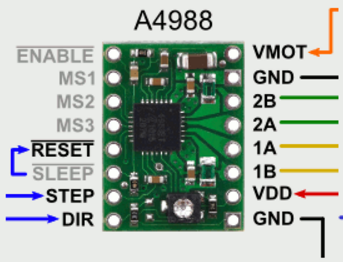
\includegraphics[scale=0.6]{tex/Implementering/Implementering_til_projektrapport/Pololu-A4988.png}}
	\caption{Pololu-A4988}
	\label{fig:Pololu-A4988}
\end{figure}

\begin{table}[H]
  \centering
\begin{tabular}{ |l|c|c|c| }
  \hline
   & \textbf{PSoC 5LP} & \textbf{Motor} & \textbf{VCC} \\
  \hline 
  ENABLE & X & & \\
  \hline
  STEP & X & & \\
  \hline
  DIR & X & & \\
  \hline
  VMOT (10V) & & & X \\
  \hline
  GND & X & & X \\
  \hline
  2B & & X & \\
  \hline
  2A & & X & \\
  \hline
  1A & & X & \\
  \hline
  1B & & X & \\
  \hline
  VCC (5V) & & & X \\
  \hline
  GND & & & X \\
  \hline
\end{tabular}
\caption{Pololu-A4988 pin konfigurering}\label{tab:Pololu-A4988_pin_configuration}
\end{table}

\noindent
VCC er altså spændingsforsyning som leverer både 5V og 10V til henholdsvis driveren og motoren.
\\
\\
Sensorerne har tre pins som alle er sat direkte til \textbf{Positionscontrolleren}, som vist i tabel \ref{tab:Sensor_pin_konfigurering}.

\begin{table}[H]
  \centering
\begin{tabular}{ |l|c| }
  \hline
  \textbf{GP2Y0A21YK Sensor} & \textbf{PSoC 5LP}\\
  \hline 
  $V_O$ & P3[1:0] \\
  \hline 
  GND & GND \\
  \hline 
  $VCC$ & VCC \\
  \hline 
\end{tabular}
\caption{GP2Y0A21YK sensor implementeret med PSoC 5LP}\label{tab:Sensor_pin_konfigurering}
\end{table}